\documentclass[a4paper,11pt,twocolumn]{article}
\usepackage{lingmacros}
\usepackage{blindtext}
\usepackage{tree-dvips}
\usepackage{amsmath}
\usepackage{multicol}
\usepackage{mathtools}
\usepackage{hyperref}
\usepackage{graphicx}
\usepackage{amssymb}
\usepackage[table]{xcolor}
\usepackage{textcomp}
\graphicspath{ {./Latex/} }
%\usepackage{wrapfig}

\begin{document}

\title{Water- and energy balance output from a simple SEB- model with varying soil depth}
\date{May 2020}
\author{Eirik Nordgård\\ Geophysical Institute,\ University of Oslo}


\twocolumn[
\begin{@twocolumnfalse}
\maketitle
\begin{abstract}
In this paper a simple bucket model has been used to model the surface energy balance and the water balance with different soil depths over a two-year period. Water level, saturation, surface runoff and energy fluxes is analysed for bucket depths of 0.1, 0.5 and 0.9 meters.  With a freezing condition prohibiting the soil water level to rise during periods of temperatures below zero, the deepest bucket almost went through the entire period without reaching saturation. The other buckets saturated quickly resulting in both surface- and subsurface runoff relatively fast after rainfall events. The soil temperature variations was greatest for the shallowest bucket, causing this bucket to experience largest fluctuations in latent heat, sensible heat, conduction and longwave radiation. 
\end{abstract}

All material used in this project may be found on 
\url{https://github.com/eirikngard/GEO4322---Surface-Energy-Balance-in-Cold-Environments}

\end{@twocolumnfalse}
]
\
\section{Introduction}

The main scope of the paper is to investigate how the water- and energy balance in a simple surface energy balance model is affected by various bucket depths. \textit{Bucket depth} is analogous to \textit{soil depth}, meaning that a bucket with water represents soil on top of bedrock on an confined area. Pouring water into the bucket beyond its capacity will cause surface runoff. This feature is modelled in its simplest way by defining the saturation of the bucket to be water level divided by bucket depth. Hence, a deeper bucket should experience less surface runoff compared to a shallow bucket. Subsurface flow is also modelled with a linear relationship to the 
\\
saturation. The surface energy balance 
is of great importance to the bucket model since it dictates the water balance by defining whether the ground is frozen or not. In reality, surface runoff may occur even if the ground is frozen, but for simplicity the model allows no surface runoff once the ground temperature is below zero. Also, the modelled surface temperature is very important as it is a key component of the turbulent fluxes and radiative terms. Keeping the energy input to a layer of soil constant should result in higher temperature for a shallow layer than a thick layer, hence making most energy fluxes into or out of a thin layer the largest. 

The paper is structured as follows. Section 2 contains theory. Section 3 describes how the model is build. Section 4 is results and section 5 is discussion. 
\
\section{Theory}


\subsection{Surface Energy Balance}

The surface energy balance is calculated for daily timesteps. Initially, the following forcing terms are given through point  measurements: Air temperature $T_{air}$, precipitation, incoming shortwave, $S_{in}$, and longwave radiation, $L_{in}$, windspeed and specific humidity.
Shortwave refelced radiation is calculated using the albedo, $\alpha$, in Eq. (\ref{eq:shortwave}).
\begin{equation}
	S_{out} = \alpha * S_{in}
	\label{eq:shortwave}
\end{equation}

Albedo is set to 0.2. Stefan-Boltzmann law is then used to calculate the longwave outgoing radiation in Eq. (\ref{eq:longwave}) \cite{dingman}.

\begin{equation}
	L_{out} = \sigma * (T_{surf}+273.15)^4
	\label{eq:longwave}
\end{equation}
where $\sigma$ is the Stefan-Boltzmann constant equal to $5.670*10^8 \; Wm^{-2}K^{-4}$ and $T_{surf}$ is the surface temperature. 

Essential to the surface energy balance is also the conductive ground heat flux between the surface with depth $d_{surf}$, and the layer below below with depth $d_{ground}$. Ideally a model should use many layers, but for simplification only one layer is used in addition to the surface layer. The conductive heat flux between the first and the second layer is calculated using Fourier's law of heat conduction:

\begin{equation}
F_{cond} = 
-K*\frac{T_{surf}-T_{ground}}{(d_{surf}+d_{ground})/2}
\end{equation}

where $K = 3 Wm^{-1}k^{-1}$ is the thermal conductivity of rock \cite{labus}. 

Sensible heat flux is calculated with Eq. (\ref{eq:sensibleheat})

\begin{equation}
Q_h = \frac{-\rho_{air}c_p\kappa^2u}{log(z/z_0)}* \frac{(T_{air}-T_1)}{log(z/z_0)}
\label{eq:sensibleheat}
\end{equation}

Potential latent heat is calculated through 
\begin{equation}
Q_{e pot} = \frac{-\rho_{air}*L_w*\kappa^2*u}{log(z/z_0)}*\frac{(q-e_s)/p}{log(z/z_0)}
\end{equation}
where the latent heat flux is dependent on saturation, $S$, and is calculated like this:
\begin{equation}
Q_e = S*Q_{e pot}
\label{eq:latentheat}
\end{equation}

In Eq. (\ref{eq:latentheat}) saturation is defined to be
\begin{equation}
S = \frac{Water Level}{Bucket Depth}
\end{equation}

To be used in the water balance, the evaporation, $Ev$, is: 

\begin{equation}
Ev = \frac{Q_e}{L_w*\rho_{water}}
\end{equation}

Now the complete energy balance is done for the surface layer \cite{dingman}  
\begin{equation}
	E_{surf} = E-S_{in}-S_{out}+L_{in}-L_{out}+F_{cond}-Q_h-Q_e
	\label{eq:surfenergy}
\end{equation}
and the second layer:
\begin{equation}
E_{ground} = E-F_{cond}
	\label{eq:groundenergy}
\end{equation}
In Eq. (\ref{eq:surfenergy}) and Eq. (\ref{eq:groundenergy}) $E$ is the energy contained in the layer from the previous timestep. Using these two energy terms and the depth, $d$, of the respective layer, one can obtain the layer temperature through Eq. (\ref{eq:layertemp}):
\begin{equation}
	T = \frac{E_{layer}}{c_h*d}
	\label{eq:layertemp}
\end{equation}

In Eq. (\ref{eq:layertemp}) $c_h = 2.2*10^6 [Jm^{-3}K^{-1}]$ is the heat capacity of rock.  


\subsection{Water Balance}
The water balance is based on conservation of mass, and describes the flow of water into and out of a closed system. This system may for example be a catchment, a lake or a column of soil. Used in areas like agriculture, runoff assessment or pollution control, making a water balance is a neat way to keep track of where the water in your system has come from and where it is going. 

To quantitatively study the water balance it is necessary to distinguish the different contributing processes. In its simplest form, the water balance can be written as \cite{dingman} 
\begin{equation}
	\Delta S = P - Ev + R_{in} - R_{out} + G_{in} - G_{out} 
	\label{eq:waterbalance}
\end{equation}

In Eq. \ref{eq:waterbalance} $P$ is precipitation, $Ev$ is evaporation, $R$ is runoff and $G$ is the groundwater flow or subsurface runoff \cite{dingman}. If several points in a grid were to be evaluated then the fluxes $R$ and $G$ should be evaluated, but for simplification neither $R_{in}$ or $G_{in}$ are considered in this model. $\Delta S$ is the resulting storage of water.    

In this model the surface energy balance becomes important as the water balance is only calculated for $T_{surf}$ and $T_{ground}$ $>=0$. This means that once the water is frozen the water balance remains unchanged. Once water is unfrozen the surface runoff $R$ in Eq. (\ref{eq:waterbalance}) is defined as
\begin{equation}
	R = max(0, P-Ev-G-d)
	\label{eq:runoff}
\end{equation}  
where $d$ is the bucket depth, simulating the total soil depth where water can be stored. It is evident from Eq. (\ref{eq:runoff}) that that surface runoff is highly dependent on the bucket depth, but also on the relative sizes of $P$, $Ev$ and $G$. In particular, one should see a increased runoff for consecutive days with heavy rainfall, especially for shallow soil.  
Once the precipitation soaks into the ground drainage becomes important. A drainage constant is set to 1.5 mm/day, implying that a deeper bucket will last longer before surface runoff occurs. 

\subsection{Forcing Data}

The simple \textit{bucket model} used in this project is dependent on forcing to function as intended. Windspeed, air temperature, rainfall, relative humidity, specific humidity, shortwave incoming radiation and longwave incoming radiation from 2nd of October 2014 to 16th of March 2019 is provided by the Applications of Research to Operations at Mesoscale (AROME) model. This convection-permitting model is a high resolution model operated by MetCoOp, an collaborative effort between the Swedish Meteorological and Hydrological Institute and the Norwegian Meteorological Institute \cite{muller}. In this study forcing data from Finse is used to force the bucket model. 

\subsection{Area}
Located at 1222 meters above sea level, on the northwestern part of the Hardangervidda plateau in Norway, Finse has a rather oceanic climate with mild winters for its altitude and cool summers \cite{finse}. Winter temperatures in the range of -20\textdegree C and summer temperatures in the range of 20\textdegree C is not uncommon. Monthly average precipitation was around 80mm between March 2019 and March 2020, peaking in September and October. Finse is very exposed to winds and frequently experiences winds in the range of 15-25 m/s \cite{yr}. 

Figure (\ref{fig:forcing}) shows air temperature and precipitation from the forcing data used in the model. Air temperatures ranges from around -25\textdegree C in winter to around 18\textdegree C in summer. Precipitation values in this dataset was extremely high, some values pushing 300 mm/day. The AROME model is known to overestimate precipitation in mountain regions and in general to overestimate large precipitation events \cite{muller}, but even taken this into account these values are extremely large for this area. One possible explanation for these high values is that all of the precipitation data points could be daily values, meaning iy is necessary to average the data points for each day. Therefore, in lack for more specific details on the data points and what units they have, a simple moving average for every day was applied for the plotting procedure. The result is shown as the black bars in Figure (\ref{fig:forcing}), showing the average daily precipitation values with maxima around 90 mm/day. These values still appear be very large compared to historical records found on yr.no \cite{yr} and seklima.no \cite{seklima}, but more correct for the area in question. Doing this dos not change the energy- or water balance in any way.

\begin{figure}[h]
	\centering 
	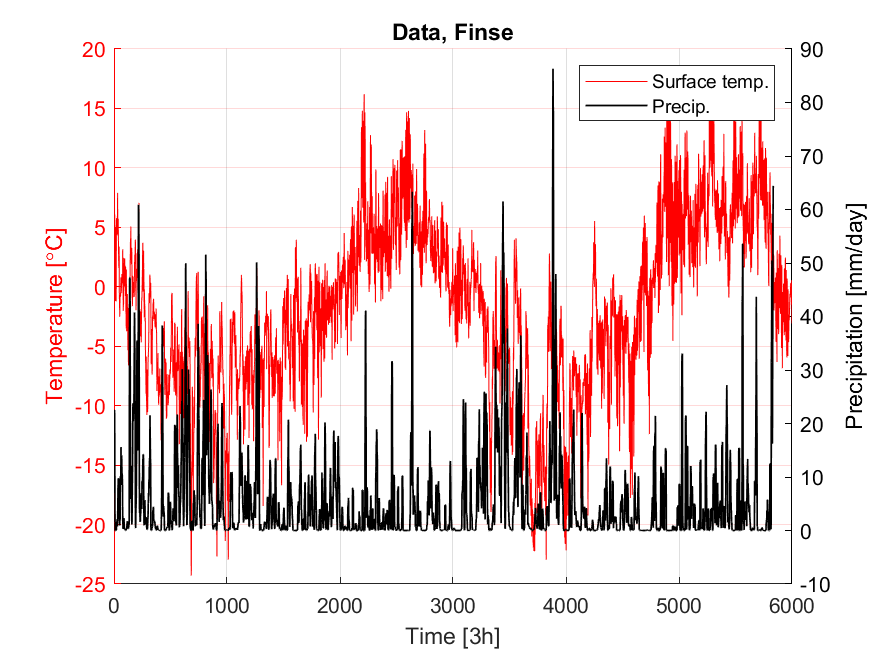
\includegraphics[width=0.5\textwidth]{figures/precip}
	\caption{Temperature (red) and precipitationv(blak) from forcing data.}
	\label{fig:forcing}
\end{figure}


\subsection{Choosing bucket depth, initial water level and drainage constant}
Choosing size of the buckets in the model is done to best simulate the actual conditions at Finse. Located at relatively high altitude with very sparse vegetation the bucket depths is set to 0.1m, 0.5m and 0.9m, one shallow, one intermediate and one deep. This selection should cover the most common range of soil depths in Finse. Initial water depth is set to 0.05m to see how the water- and energy balance evolves from a relatively dry soil cover. Drainage constant is set to 1.5 mm/day. This is a guessed mean value for all bucket depths.    


\section{Model Build}

Being a very simple surface energy balance model, it is essentially build within two for-loops and a simple if-statement. Outermost is the loop iterating over the different bucket depths. Within is all necessary constants defined. Thereafter the surface energy balance and water balance is calculated for each timestep. The model is designed to develop surface- and subsurface runoff, but only if the temperature of the two soil layers are above freezing. Scripts associated with the model can be found in the GitHub link provided on the first page of the paper.         

\section{Results}

As many of the fluxes in the model is somehow dependent on the surface temperature, it should be the controlling factor for most of them. The surface temperature varies from around -25\textdegree C in winter to around 32\textdegree C in summer as shown in Figure (\ref{fig:t1}). There are greatest temperature variations in the smallest bucket. Overall difference in surface temperature between the different buckets is very small, not greater than around 3\textdegree C from the deepest to the shallowest in most cases. Also, the daily surface temperature variations are far greater during summer than winter.  

\begin{figure}[h]
	\centering 
	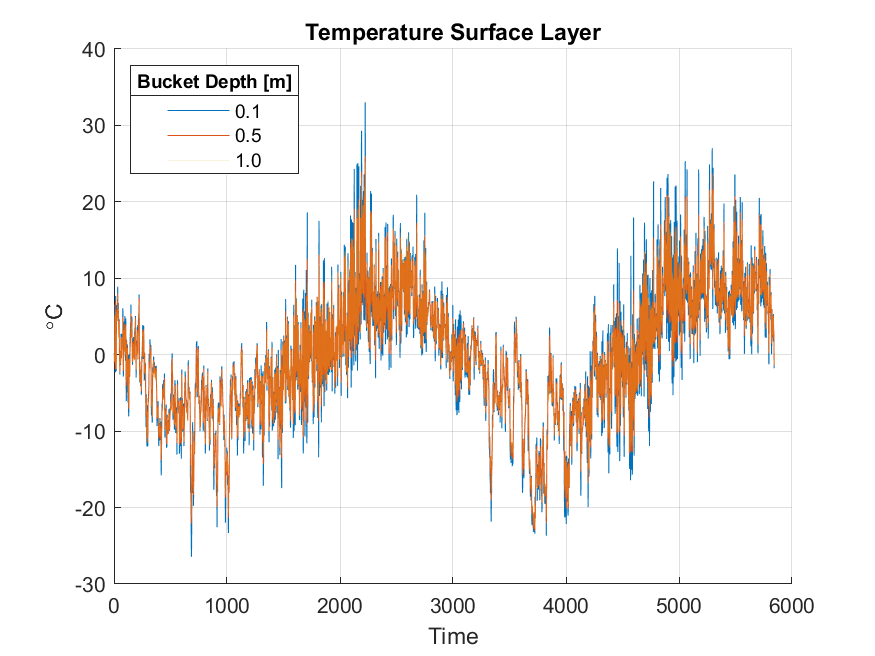
\includegraphics[width=0.5\textwidth]{figures/t_surface}
	\caption{Surface temperature with varying bucket depth.}
	\label{fig:t1}
\end{figure} 

Interestingly the temperature of the second layer is very different when it comes to the different buckets compare to the surface layer. Figure (\ref{fig:t2}) indicates that the shallowest bucket appear to have fluctuations very close to that of the surface layer, but in the deeper buckets the temperature variations are drastically damped. For the shallowest bucket the daily temperature difference is close to 10 \textdegree C in most cases, while the deepest bucket only experiences daily variations around 1\textdegree C.     

\begin{figure}[h]
	\centering 
	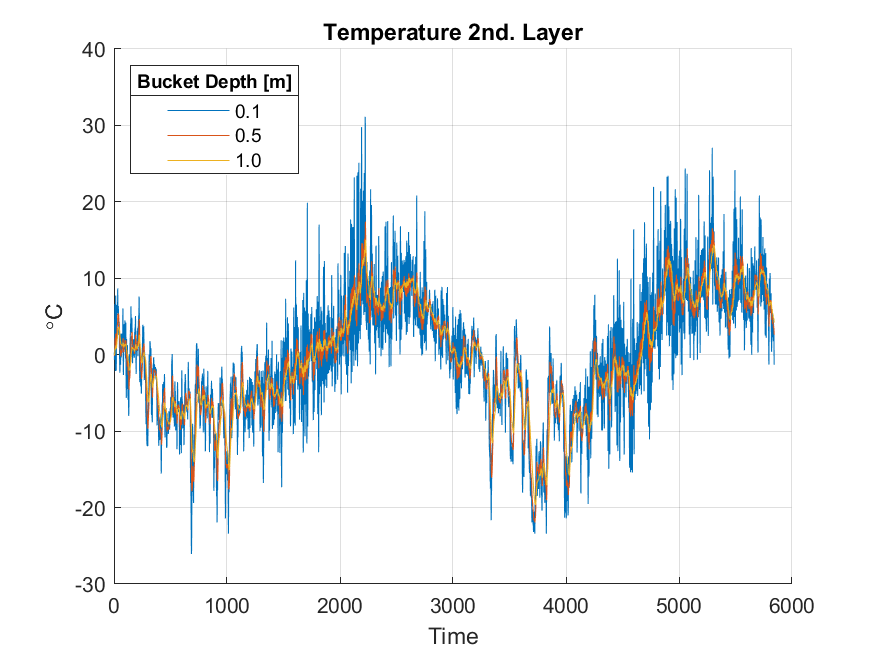
\includegraphics[width=0.5\textwidth]{figures/t_ground}
	\caption{Temperature of 2.nd layer with varying bucket depth.}
	\label{fig:t2}
\end{figure} 


Values of latent heat ranges from -200 to almost 500 $W/m^2$ in accordance with Figure (\ref{fig:latent}). The values are in general a lot higher during summer than during winter. This is expected since the summer temperature is much higher than the winter temperature. There are no apparent reaction in latent heat to the precipitation events although actual latent heat should spike after precipitation events. Although increased soil saturation should have substantial impact on the evaporation, but this process may be to fast in reality to be properly captured by this model. Modelled soil saturation increases after precipitation events, but the direct surface evaporation appears to be poorly captured by the model. In general the shallowest bucket experiences strongest evaporation and hence the largest latent heat flux. A shallow bucket allows for quick saturation which in turn enhances evaporation in the model.

\begin{figure}[h]
	\centering 
	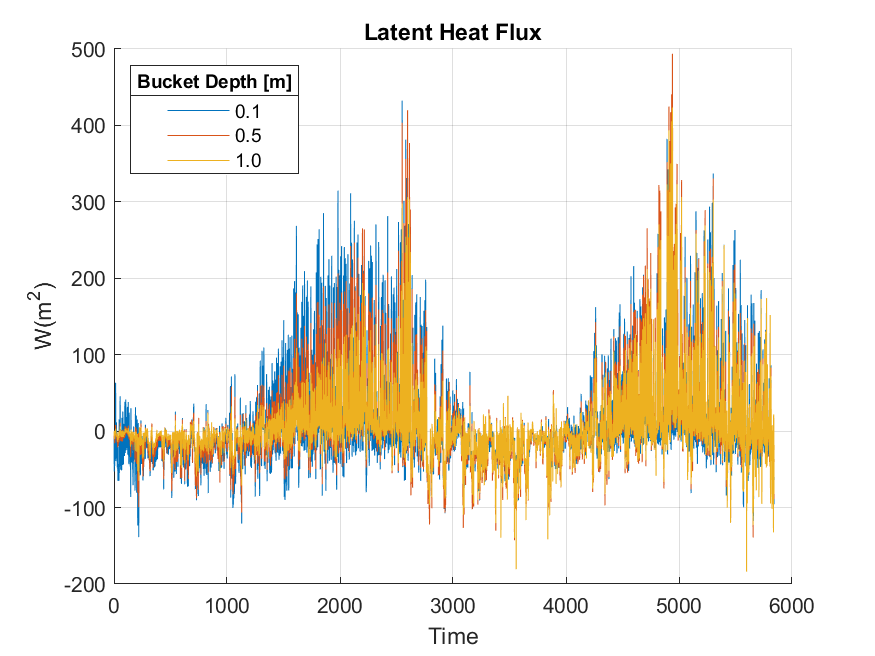
\includegraphics[width=0.5\textwidth]{figures/latent_heat}
	\caption{Latent heat with varying bucket depth.}
	\label{fig:latent}
\end{figure} 

During summer and early autumn the shallowest bucket has largest negative sensible heat flux values, while the deepest bucket has the largest positive values. During winter the largest negative sensible heat values are found with the deepest bucket while the largest positive values are a blend from the shallower buckets. Values ranges from 300-500 $W/m^{2}$ in summertime to - 200-300 $W/m^{2}$ in wintertime as shown in Figure (\ref{fig:sensible}). Positive flux is heat loss from the surface and negative value are heat gain to the surface. A deep bucket can potentially store more heat compared to a shallow bucket, explaining why the flux is larger for the deepest bucket in winter. 
%Q_h(Tair, T_1, windspeed)  

\begin{figure}[h]
	\centering 
	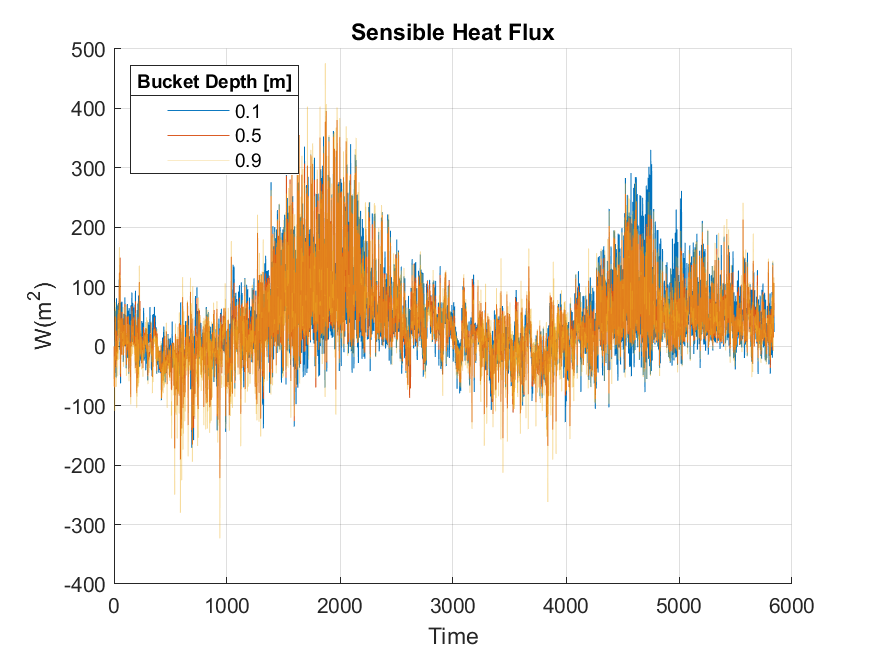
\includegraphics[width=0.5\textwidth]{figures/sensible_heat}
	\caption{Sensible heat with varying bucket depth.}
	\label{fig:sensible}
\end{figure} 

In the shallow bucket the surface temperature reacts to the air temperature quicker than with a deeper bucket, meaning that in a deeper bucket the surface temperature is less affected by the air temperature since the entire bucket has a lower temperature. Hence the flux from the air to the ground in winter is largest for a deep bucket. During summer nights the thin layer of soil looses heat to the air quickly making a large positive flux, while during the day the thin layer of soil is heated rapidly making a large negative flux. Both of these processes reqers more time for a deeper bucket. 

The heat flux through conduction is  positive from the second layer up to the surface layer and vice versa. It ranges between 250 and -250 $W/m^2$ and is largest is summertime as displayed in Figure (\ref{fig:conduction}). Shallow buckets have the largest values, both positive and negative while the deepest bucket have more modest values between 50 and -50 $W/m^2$. This is a direct consequence of the that fact that the shallow bucket has higher temperature compared to the deeper bucket. More available energy allows for more energy to be conducted to the surrounding layer of soil.

\begin{figure}[h]
	\centering 
	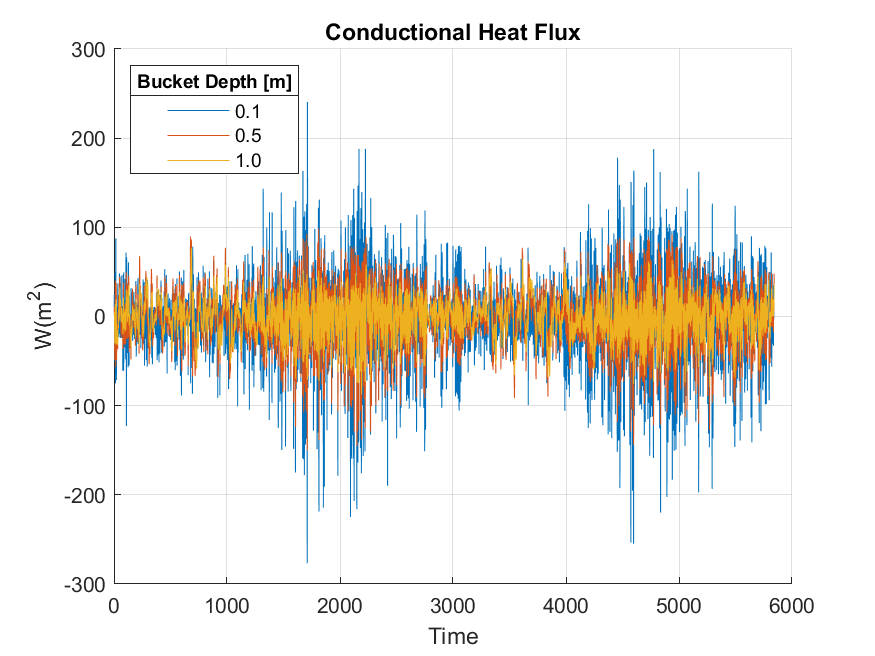
\includegraphics[width=0.5\textwidth]{figures/conduction}
	\caption{Conduction with varying bucket depth.}
	\label{fig:conduction}
\end{figure} 

Longwave outgoing radiation varies from 200 to 500 $W/m^2$. It is larger in winter than in summer, which is explained by the higher summer surface temperatures. The different buckets produce a very similar flux in winter, while in summer the flux varies with around 30 $W/m^2$ from the shallowest to the deepest bucket. Like for the conduction the shallowest bucket generally produces both the largest and the smallest flux. This is once again expected as the longwave outgoing flux is determined by the Stefan Boltzman law which is dependent on the surface temperature. 

Moving over to the water balance Figure(\ref{fig:bucket_fixed}) shows how the water level is rising and dropping with time. The flat parts of the curve have two physical interpretations. Firstly, the surface temperature may be below zero, freezing the entire water balance. Secondly,the bucket may have become saturated and is unable to store more water. A flat water level curve from start for the shallowest bucket indicates that this saturates very fast. The other two buckets quickly fills but flattens before saturation due to freezing. From Figure(\ref{fig:bucket_fixed}) we one can also observe that the deepest bucket not saturates before the very end of the two-year period while the 0.5 meter bucket saturates after the first summer. 

\begin{figure}[h]
	\centering 
	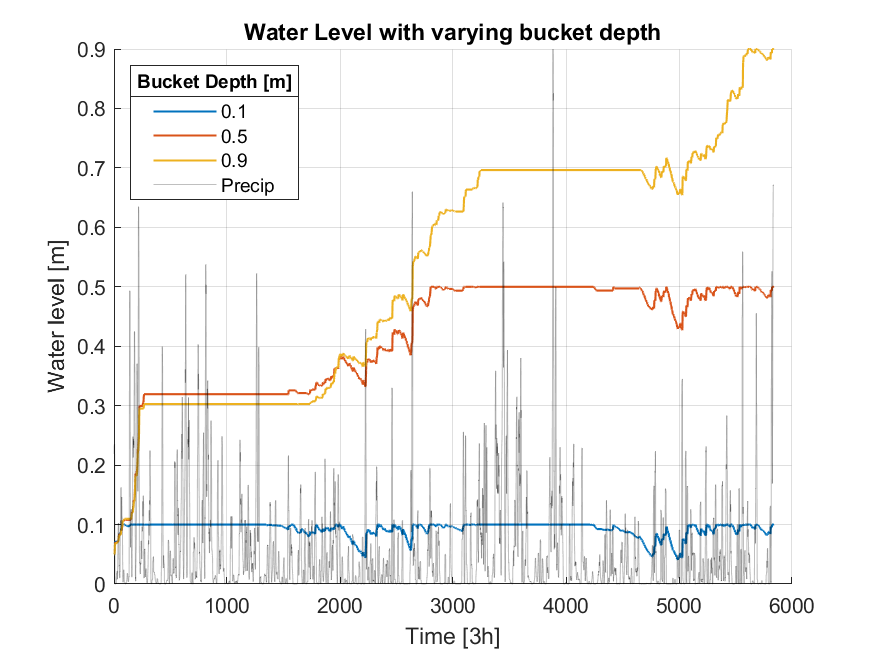
\includegraphics[width=0.5\textwidth]{figures/bucket_depth_fixed}
	\caption{Water level in soil dependent on the bucket depth.   Gray line is precipitation for reference.}
	\label{fig:bucket_fixed}
\end{figure}

Since all of the buckets eventually reaches saturation, surface runoff will occur as shown in Figure (\ref{fig:runoff}). The runoff values are relatively high compared to the precipitation values, apparently being close to the full size of the precipitation event. Each of the buckets experiences runoff where one deeper bucket also experiences runoff. Towards the end of the plot in Figure (\ref{fig:runoff}) it may look like only the deepest bucket experiences runoff, but since the deepest bucket experiences runoff at this point in time, all of the other buckets also experiences runoff here.  

\begin{figure}[h]
	\centering 
	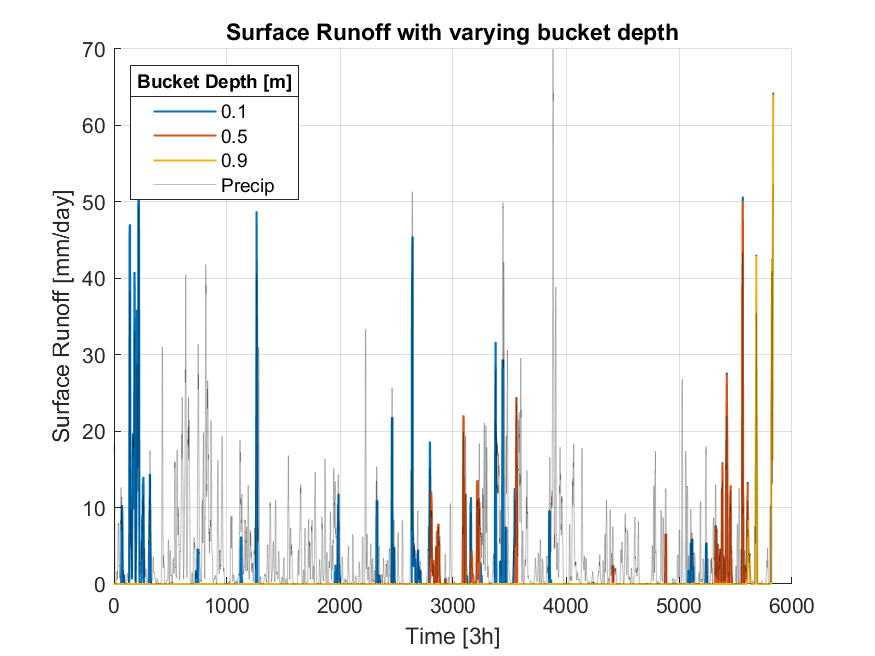
\includegraphics[width=0.5\textwidth]{figures/runoff}
	\caption{Surface runoff with varying bucket depth. Gray line is precipitation for reference.}
	\label{fig:runoff}
\end{figure} 

\section{Discussion}

Overall the modelled energy- and water balance appear to fit the actual conditions at Finse quite well. None of the modelled fluxes are surprisingly large or small. Modelling these balances with different soil depths proved to showcase some interesting features of the water- and energy balance.  

One strange feature of the model is that the water level appears to be rising and rising throughout the two-year period. This is certainly not the case in the true world as and may indicate that the deepest bucket is actually too deep to represent this area. This might also be an effect of other parameters in the model being chosen too large or too small. Increasing the drainage constant would solve this problem, but on the other hand this might cause the shallow buckets to drain too fast. It may also be caused by missing drainage features in the model such as streams and creeks moving water through or away from the soil. 

One obvious shortcoming of the model is the simplification of the water balance once the ground temperature in both layers drops below freezing. Since this simplification applies to the periods of the year where the fluxes of water and energy generally not are huge, it might be the case that the actual balances are not altered too much. Despite this some details in the balances may be left out of the picture. Processes like snow infiltration and refreezing of water is not captured by this model. These factor are some out of several that might change the properties of surface runoff and evaporation to mention some. 

Additionally, snow and snowcover is not included in the model. Snow has a great impact on the surface energy balance because of its reflecting abilities. With an high albedo compared to bare soil or rock, snow will reflect most of the incoming shortwave radiation. This drastically reduces the amount of available energy to the environment, hence reducing energy available for evaporation and the sizes of the sensible and latent heat flux. Also, at Finse a lot of the precipitation used in this model falls as snow rather than rain. Including this would further implicate the energy balance since less liquid water would be available for evaporation, and more energy would be spent to melt snow towards the summer month. A suggestion to improvement of this simplified model would be to incorporate the effect of snow to see how the different buckets are affected in terms of the water- and energy balance.
\twocolumn
[
\begin{@twocolumnfalse}


\medskip

\begin{thebibliography}{9}

\bibitem{dingman}
Dingman S. Lawrence \\
\textit{Physical Hydrology}\\
Third Edition \\
Waveland Press, 2015.\\

\bibitem{labus}
Labus, M., Labus, K. Thermal conductivity and diffusivity of fine-grained sedimentary rocks. J Therm Anal Calorim 132, 1669–1676 (2018). \\
URL: \url{https://doi.org/10.1007/s10973-018-7090-5}

\bibitem{muller}
MÜller et al. 2017\\
\textit{AROME-MetCoOp: A Nordic Convective-Scale Operational
Weather Prediction Model}\\
URL: \url{https://doi.org/10.1175/WAF-D-16-0099.1}

\bibitem{finse}
Webpage of Finse Alpine Research Ceenter\\
URL: \url{https://www.finse.uio.no/about/location/}\\
Visited 20th of April 2020

\bibitem{seklima}
Historical precipitation records from Finse.\\
URL: \url{https://seklima.met.no/observations/}

\bibitem{yr}
Webpage of Nowegian forcasting service YR for historical data for Finse.\\
URL: \url{https://www.yr.no/nb/historikk/graf/1-111123/Norge/Vestland/Ulvik/Finse}


\end{thebibliography} 


\end{@twocolumnfalse}
\
]

\end{document}